\chapter{Private-Key Cryptography}

\section{One Time Pad}

The One Time Pad works as follows:

\begin{enumerate}
    \item Alice has a message $m \in \{0,1\}^n$ to be sent to Bob. Furthermore, Alice and Bob possess a common key $k \in \{0,1\}^n, n\in N$. $n$ is called the security parameter.
    \item Alice computes a cipher text $c \in \{0,1\}^{n}$ as $c = m \oplus k$ and sends it to Bob.
    \item Bob reconstructs the plain message as $m = c \oplus k = m \oplus k \oplus k = m \oplus \{0\}^{n}$.
\end{enumerate}

Therefore, the abstract object for this cryptographic process consists of the following functions\footnote{The symbol $\perp$ is indicating an error.}:

\begin{itemize}
    \item $kGen(1^{n}) \rightarrow k \in \{0,1\}^{n}$
    \item $enc(m, k) \rightarrow c, \quad |m| = |k| = |c| = n$
    \item $dec(c, k) \rightarrow m \quad || \quad \perp$
\end{itemize}

The functional correctness is then defined as follows:\\
For all security parameter $n \in N$, for all messages $m$, for all keys $k \leftarrow kGen(1^{n})$, for all keys $k \leftarrow kGen(m,k)$ and for all ciphertexts $c \leftarrow enc(m,k)$ applies $dec(c,k) = m$. That means that we must be able to decrypt all encrypted messages for all possible input parameters.

\subsection*{Security of Shannon's OTP}

Independently of a bit $m_i$ in the message $m$, the OTP flips this bit with the probability of $\frac{1}{2}$ creating a distribution of ciphtertexts $c$ that is independent of the messages $m$. And because $m$ and $c$ are independent, it is intuitive that knowing $c$ cannot reveal anything about $m$. We can also prove this mathematically because the probability for two independent events to take place is the product of the individual probabilities: $Pr[M=m | C=c] = \frac{Pr[M=m \wedge C=c]}{Pr[C=c]} = \frac{Pr[M=m] \cdot Pr[C=c]}{Pr[C=c]} = Pr[M=m]$.


\section{Practical security}

In practice, perfect security is not feasible because this would mean that for transferring each message $m$ a key $k$ with at least the same length $|k| \geq |m|$ would have to be transferred (see definition of perfect security in section \ref{sec:gloss:perf_sec}). For this reason, we define a weakened security definition, which comes in two variants \textendash{} Concrete security and asymptotic security. In this course, we look at asymptotic security.

\begin{tabular}{|p{0.47\linewidth}|p{0.47\linewidth}|}
    \hline
    \textbf{Concrete Security:}                                                                                                       & \textbf{Asymptotic Security}                                                                                                                                          \\
    \hline
    A process is $(t,\mathcal{E})$-secure if no attacker $A$ can break it with at most $t$ steps with a probability of $\mathcal{E}$. & A process is secure, if no efficient (polynomial limited by security parameter $n$) algorithm breaks it with non-negligible (less than $\frac{1}{poly}$) probability. \\
    \hline
\end{tabular}

The relevant terms are defined as follows, where $n$ is the security parameter (e.g. key size):

\begin{itemize}
    \item \textit{Efficient Algorithm:} Algorithm with polynomial runtime with regard to $n$.
    \item \textit{Non-negligible Probability:} An inversely polynomial probability ($\frac{1}{poly}$) with regard to $n$.
    \item \textit{Negligible Probability:} Smaller than an inversely polynomial function (i.e. less than non-negligible) $\leq \frac{1}{poly}$. Mathematically speaking, a function $\mathcal{E} \coloneqq N \rightarrow R$ if there can be found a value $limit \in N$, such that for all polynomial functions $poly$ applies $\mathcal{E}(n) \leq \frac{1}{poly} \quad|\quad n \ge limit$. This means that, if the security parameter is high enough, its value is smaller than any polynomial function. Stating that a function $\mathcal{E}$ is negligible can be written in three ways: $\mathcal{E} \leq neg(n)$, $\mathcal{E} = neg(n)$ or $\mathcal{E} \approx 0$. Furthermore, if a the function $\mathcal{E}_{1}$ and the function $\mathcal{E}_{2}$ differ by a negligible difference, we can write $\mathcal{E}_{1} \approx \mathcal{E}_{2}$.
\end{itemize}

\subsection*{Examples for Negligibility of probability functions}

\begin{itemize}
    \item $\mathcal{E} = 2^{-n}$ is \textit{negligible} because exponential functions grow faster than polynomial functions.
    \item $\mathcal{E} = n^{-5}$ is \textit{not negligible} because there are polynomials that have smaller values as n approaches infinity e.g. $n^{-6}$.
    \item $\mathcal{E} = \begin{cases}
                  2^{-n} & \text{if $n$ is even}   \\
                  n^{-5} & \text{if $n$ is uneven}
              \end{cases}$
          is \textit{not negligible} because for some values (all uneven values) it behaves like a polynomial function, such that e.g. $n^{-6}$ would have greater values regardless of a chosen $limit$.
    \item $\mathcal{E} = \frac{1}{8}$ is \textit{not negligible} because it does not approach zero and therefore there are many polynomial functions that are smaller than $\mathcal{E}$ for high $n$
\end{itemize}

\subsection*{Arithmetic Laws for Negligible Functions}

If $mathcal{E}_{1}$ and $mathcal{E}_{2}$ are negligible functions $mathcal{E}_{1}, mathcal{E}_{2} \approx 0$ and $q$ is a polynomial function $q = poly$ and $\omega$ ia a non-negligible $\omega \not\approx 0$ function, then applies:

\begin{align}
    \mathcal{E}_{1}(n) + \mathcal{E}_{2}(n) & \approx 0     \label{eq:neglig_1}        \\
    \mathcal{E}_{1}(n) \cdot q(n)           & \approx 0            \label{eq:neglig_2} \\
    \omega(n) - \mathcal{E}_{1}(n)          & \not\approx 0 \label{eq:neglig_3}
\end{align}

More intuitively phrased:

\begin{enumerate}
    \item[(\ref{eq:neglig_1})] Executing a negligible function and another negligible function after each other will still result in something negligible.
    \item[(\ref{eq:neglig_1})] Executing a negligible function for any polynomial number of times will still result in a negligible value in sum because the negligible function approaches zero faster than any polynomial function could grow towards positive values.
    \item[(\ref{eq:neglig_1})] Subtracting something negligible from something non-negligible does not make a difference \textendash{} the result is still non-negligible.
\end{enumerate}

\subsection{Semantic Security \textendash{} A Simulation-Based Definition}
\label{sec:semantic_securits}

A cryptographic process is semantically secure if for all PPT attacker algorithms $A$, which calculate information $f(m)$ about a length-invariant message $m$ (message of given length $n$) with the help of the message's ciphertext $c$ with a certain probability, there is a simulator algorithm $S$, which can compute the same information with a negligibly different probability:

$$
    Pr[A(1^{n},c) = f(m)] \approx Pr[S(1^{n}) = f(m)]
$$

More intuitively speaking, everything which can be computed with the knowledge about the ciphtertext of a message can also be computed with nearly the same precision without knowledge about the ciphertext.

This is the simulation-based definition of asymptotic security.

\subsection[Indistinguishability (IND) \textendash{} a Game-Based Definition]{Indistinguishability (IND) Security \textendash{} a Game-Based Definition}

This is a game-based definition of asymptotic security, which is equivalent to the semantic security definition (\ref{sec:semantic_securits}).

A cryptographic process $\mathcal{E}$ is indistinguishable (IND) if for all PPT attackers $A$ applies:

$$
    Pr[Exp_{\mathcal{E}, A}^{IND}(n) = 1] \approx \frac{1}{2}
$$

, where $Exp_{\mathcal{E}, A}^{IND}(n)$ is defined as the following algorithm:

\begin{align}
    KGen(1^{n})   & \rightarrow k                                       \label{eq:ind:keygen}      \\
    \{0, 1\}      & \rightarrow b             \label{eq:ind:choose_b}                              \\
    A(1^n)        & \rightarrow (st, m_0, m_1) | \quad |m_0| = |m_1| = n \label{eq:ind:choose_msg} \\
    Enc(m_b, k)   & \rightarrow c                          \label{eq:ind:enc_msg}                  \\
    A(1^n, st, c) & \rightarrow   \label{eq:ind:decide}                                  a         \\
    return \quad a == b \label{eq:ind:ret}
\end{align}

More intuitive worded, this means that (\ref{eq:ind:keygen}) a secret key of length $n$ is chosen (\ref{eq:ind:choose_b}) a secret random bit is chosen (\ref{eq:ind:choose_msg}) the attacker selects two messages of his choice (\ref{eq:ind:enc_msg}) one through $b$ randomly selected message is encrypted (\ref{eq:ind:decide}) the attacker looks at the ciphertext of one of its messages and decides which messages ciphertext that is and (\ref{eq:ind:ret}) the experiment returns true if the attacker has been able to identify the message and otherwise false. If the output of this experiment is negligible close to $\frac{1}{2}$ for all attackers $A$, then the attackers have no significant advantage over simply guessing and, therefore, the cryptographic process $\mathcal{E}$ is secure.

An example of an insecure process $\mathcal{E}$ could be an algorithm, which simply flips all bits: $Enc(m, k) = \thicksim(m)$. The attacker could then just use the $Enc$ algorithm (which is not secret) with any key and get the same result because the $Enc$ algorithm does not use the key. Therefore, he could distinguish messages with the probability of $1 \not\approx \frac{1}{2}$.

An example of a secure algorithm is Shannon's OTP. The reason is that without knowing the key, the attacker cannot distinguish two messages, because the OTP flips bits with the probability of $\frac{1}{2}$, such that the cipthertext is completely random, just like the key.


\section{Pseudo Random (Number) Generators (PR(N)G)}

An algorithm $G$ is a secure PRG, if for all PPT attackers $A$ applies:

$$
    Pr[Exp_{G,A}^{PRG}(n) = 1] \approx \frac{1}{2}
$$

, where $Exp_{G,A}^{PRG}(n)$ is defined as:

\begin{align}
    KGen(1^n)        & \rightarrow k   \\
    \{0, 1\}         & \rightarrow b   \\
    G(k)             & \rightarrow y_0 \\
    \{0, 1\}^{|y_0|} & \rightarrow     \\
    A(1^n, y_b)      & \rightarrow a   \\
    return           & \quad a == b
\end{align}

More intuitively speaking, this means if we generate a pseudo-random bitstring $y_0$ using $G$ and a fully random bitstring $y_1$, no attacker algorithm can distinguish them.

There is another definition of PRG, where the secret bit $b$ is set from the beginning. In this case the experiment will not return the expression $a==b$ but instead directly return the attacker's guess $a$. The IND security of the PRG is then defined as follows: The behavior of the attacker (i.e. its return value) is not significantly influenced by whether we give it the output of the PRG or a random bitstring (i.e. it does not depend on the value b):

$$
    Pr[Exp_{G,A,0}^{PRG}(n) = 1] \approx Pr[Exp_{G,A,1}^{PRG}(n) = 1]
$$

As a side note, following Kerckhoff's principle, a potential attacker could also access our PRG. He could, therefore, calculate the pseudo-random strings for all possible input values in $|K_n|$. This means, that a generated value $y$ only has the security of $2^k$ instead of $2^{|y|}$. However, as $|K_n|$ grows exponentially, such an attacker would not be efficient and is, therefore, asymptotically irrelevant.

\section{PRGs for Key Expansion}

We have seen that the OTP is not practicable because for using it we must first exchange a key that is just as long as the message itself. Now that we have looked into PRGs from an abstract point of view, we could use PRGs to generate a long key from a small key and then use that for encryption:

\begin{align}
     & KGen(1^n) \rightarrow k             & |\quad   & n \in \{0,1\}^n              \\
     & Enc(k,m)  \rightarrow m \oplus G(k) & |  \quad & M_n=\{0,1\}^{l(n)}           \\
     & Dec(k,c)  \rightarrow c \oplus G(k) & or \     & \perp if \ |c| \ \neq \ l(n)
\end{align}

Given the assumption that the Generator $G$ is IND-secure, we must now prove that the encryption method $\mathcal{E}$, which utilizes it, is also secure. A suitable method of proof for this is reduction.\\
\textbf{The main idea of using reduction for proving the IND security of a cryptographic method $\mathcal{E}$ is the following:}

Assume that $\mathcal{E}$ is not IND-secure and, therefore, we could find an attacker algorithm $A_{\mathcal{E}}$ which breaks $\mathcal{E}$. Then construct a new attacker $A_{\mathcal{E}'}$ utilizing $A_{\mathcal{E}}$, which breaks another cryptographic method $\mathcal{E}'$, which is known to be secure. The existence of the newly constructed attacker would then contradict the knowledge about $\mathcal{E}'$. Hence, $\mathcal{E}$ must be IND-secure.

To prove the IND security of the newly constructed cryptographic method $\mathcal{E}$ we reduce it to the IND-security of the utilized PRG as shown in figure \ref{fig:reduction_key_expansion}. We have a PRG challenger that challenges us to decide if its output is a random number or the output of the PRG. Then we take the challenger's output $y_b$ and use it to compute a ciphertext $c$ of a randomly chosen message. Assuming the PRG challenger gives us $y_0$, what we did until now is exactly what a challenger of an IND experiment for $\mathcal{E}$ would do. Because we assume that $\mathcal{E}$ is not IND-secure, the attacker $A_{\mathcal{E}}$ will then be able to efficiently decide what message has been encrypted by us (choose x == a). But in case the PRG challenger gives us $y_1$, the process of creating $c$ is equivalent to an OTP, which we know is IND-secure, and can therefore not be decided by $A_{\mathcal{E}}$. That means, if there was an efficient attacker for the IND experiment for $\mathcal{E}$, this reduction would build an efficient IND attacker for the PRG. Hence, given the fact the PRG is IND secure, this would contradict. It follows that $\mathcal{E}$ is IND secure if the used PRG is IND secure and otherwise not.

\begin{figure}
    \center
    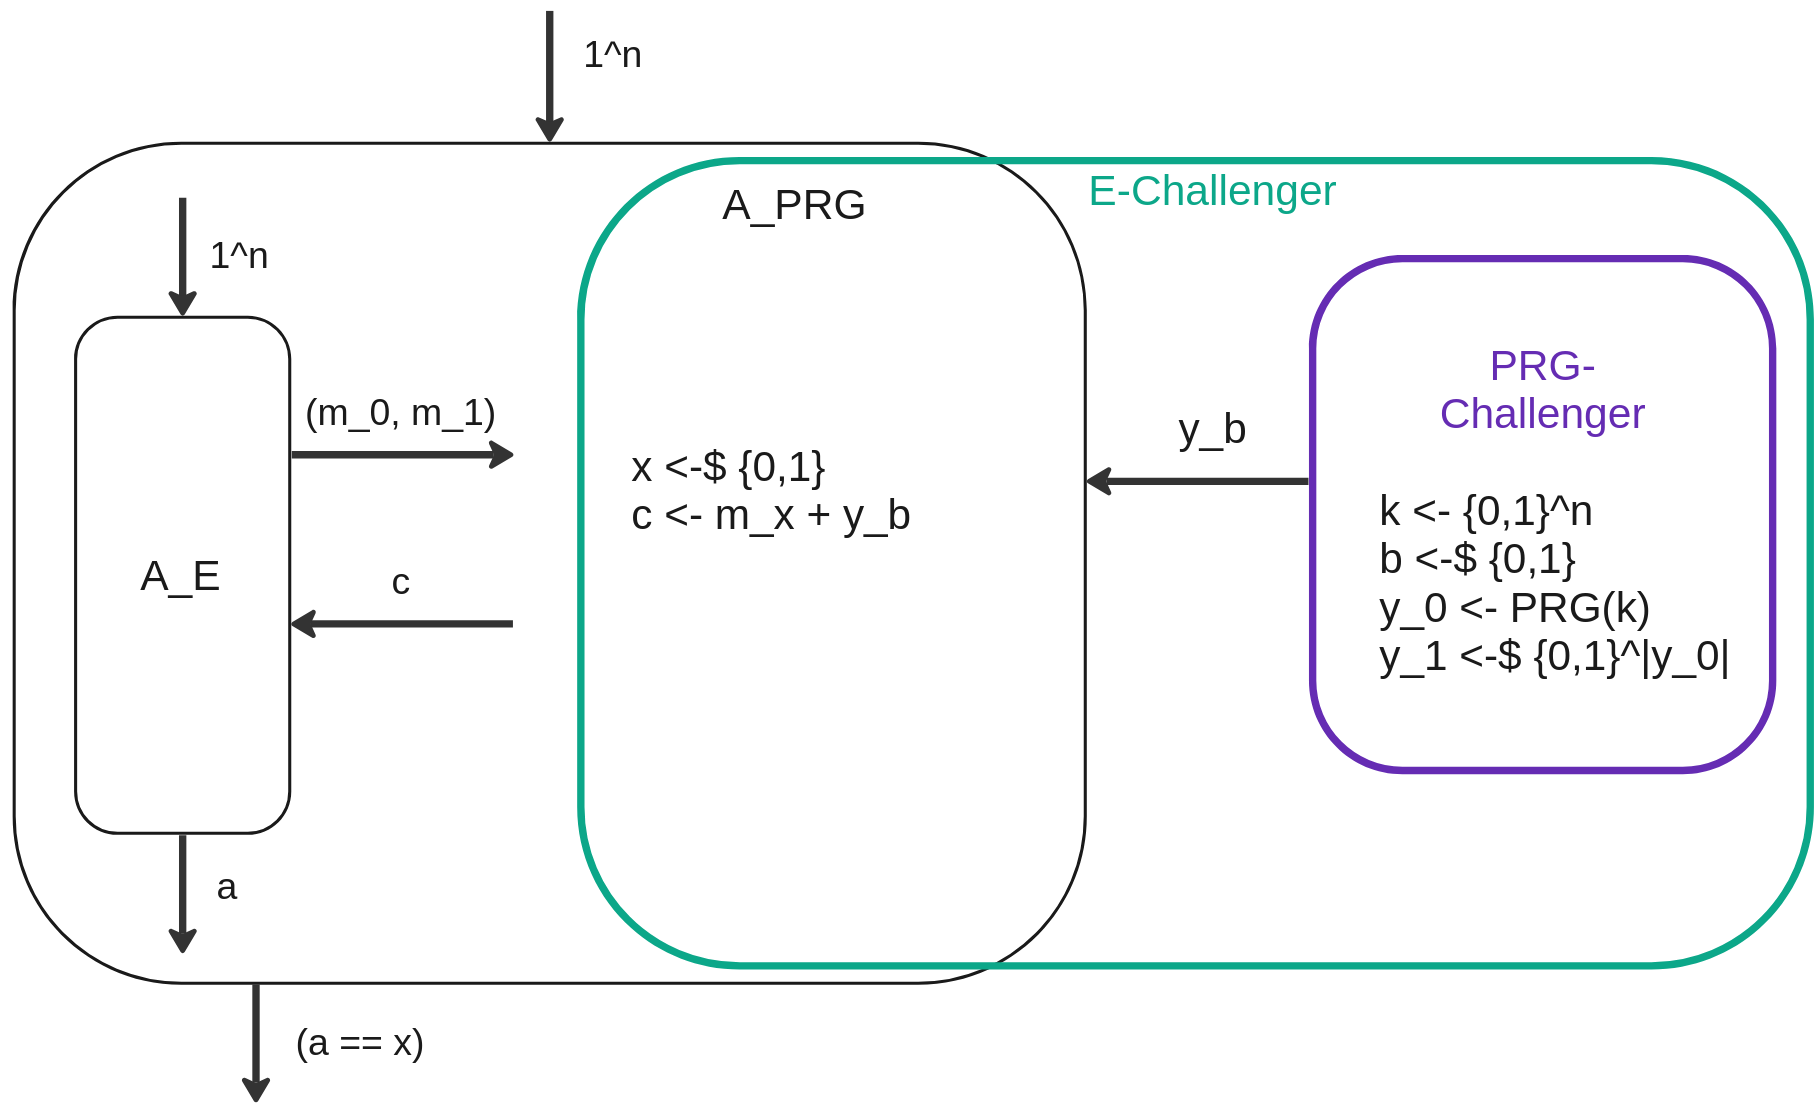
\includegraphics[width=\linewidth]{gfx/reduction_prg_key_expansion.png}
    \caption{Reduction for proving the IND-security of $\mathcal{E}$ if the IND-Security of PRG is given.}
    \label{fig:reduction_key_expansion}
\end{figure}


\section{Indistinguishability Under Chosen Plaintext Attack (IND-CPA)}

CPA is an attack model in which the attacker can retrieve ciphertexts for arbitrarily chosen plain texts as many times as he wants. But because the attacker must be efficient, he can just retrieve a polynomial amount of ciphertexts. The game-based definition of IND-CPA security is identical to the definition of IND security but allows requesting $c_b$ multiple times for different message pairs $(m_0, m_1)$. But the encryption oracle will have to choose $b$ once in the beginning and then keep it the same for each request.

Every IND-CPA-secure method is also IND-secure. But IND-secure methods are not automatically IND-CPA secure. For example, the OTP with the same key for each message is IND secure but not IND-CPA secure: An attacker could request the ciphertext for two message pairs $(m_0, m_1) \rightarrow c_1$ and $(m_0, m_2) \rightarrow c_2$. The attacker knows that if $b=0$, the oracle has encrypted $m_0$ two times and will therefore return $0$ if $c1 == c2$. If $b=2$, the oracle must have encrypted two different messages, which must because of correctness be mapped to different ciphertexts. Therefore, the attacker returns $1$ if $c_1 \neq c_2$.

An approach for making an encryption method using a secure PRG IND-CPA secure could be the following:\\
For each message to encrypt, call the PRG first to generate a key that is twice as long as the fixed-size message length. Then use the first half of the PRG output for encryption and save the second part. The first seed for the PRG will be taken from a $KGen$ algorithm. The following keys will be the second half of the PRG in the previous iteration. Because the PRG output is pseudo-randomized, it is also a secure seed.\\
This approach is nice, but it is not practicable, because the sender and the receiver must be synchronized, which might fail because of insecure connections with message retransmissions.

%%%%%%%%%%%%%%%%%%%%%%%%%%%%%%%%%%%%%%%
\section{Pseudo Random Functions (PRF) (Exercise 5)}
%%%%%%%%%%%%%%%%%%%%%%%%%%%%%%%%%%%%%%%

A PRF $PRF :=  K \times \{0,1\}^{in(\gamma)} \rightarrow \{0,1\}^{out(\gamma)}$ is a family of functions. When choosing a concrete $k$, the resulting function $f \in F$ is a pseudo-random function. For different key values, the function behaves like a different pseudo-random function.

Another way to explain this is that a PRF is a function $F(k,x) \rightarrow y$, which takes a (secret) key and a seed an $x$-value as input and produces a pseudo-random output with the following characteristics:

\begin{itemize}
    \item $y_0$ and $y_1$, generated as $F(k,x_0) \rightarrow y_0$ and $F(k,x_0) \rightarrow y_0$, are different, if $x_0 \neq x_1$ and are equal if $x_0 = x_1$.
    \item A CPA attacker cannot distinguish the output of a PRF from a truly random function, which would do the same thing but in a truly randomized fashion.
\end{itemize}

A PRF with equal input and output length is called length-preserving.

Defining a (secure) PRF using a game would involve creating a challenger which randomly chooses a hidden bit $b$ and, depending on that bit, calls the PRF or a truly random function. For both, the truly random function and the PRF, the outputs must be deterministic (consistent), such that if the same $x$ value is provided as input, the same $y$ value will be emitted.

%%%%%%%%%%%%%%%%%%%%%%%%%%%%%%%%%%%%%%%
\section{Pseudo Random Permutations (PRPs) (Exercise 6)}
%%%%%%%%%%%%%%%%%%%%%%%%%%%%%%%%%%%%%%%

A pseudo-random permutation is, similar to a pseudo-random function, a family of functions, which a concrete function can be selected from by choosing a key. A pseudo-random permutation is defined as $\{0,1\}^s \times \{0,1\}^l \rightarrow \{0,1\}^l$ with the key length $s$, and the input and output length $l$. The input space and the output space of a PRP are equal and the PRP defines a bijective permutation on the set of input bit strings (not on the set of input bits), making a PRP an invertible function. In other words, every possible bitstring is mapped to another bitstring of the same length. Each output bitstring belongs to exactly one input bitstring. Every PRP is a length-preserving PRF.

A \textit{secure} (weak \textit{PRP}) is defined just like the definition for the secure PRF (as it is also a PRF).

In contrast to PRFs and PRGs, PRPs also have a \textit{strong} security definition.
A PRP is strong if is secure under chosen plain text attacks if the attacker can access the PRP and its inverted operation PRP$^{-1}$.
The game-based CPA-IND definition states that, for a chosen bitstring, a distinguisher $D$ cannot distinguish the PRPs output of $f(x)$ or $f^{-1}(x)$ from the output of a real random permutation or its inverse operation.

%%%%%%%%%%%%%%%%%%%%%%%%%%%%%%%%%%%%%%%
\section{Data Encryption Standard (DES)}
%%%%%%%%%%%%%%%%%%%%%%%%%%%%%%%%%%%%%%%

DES is a block cipher, which was used until about the year 2000. Because of its short keys, it was later replaced with DES3 and eventually by AES.

\begin{wrapfigure}{r}{0.33\textwidth}
    \begin{center}
        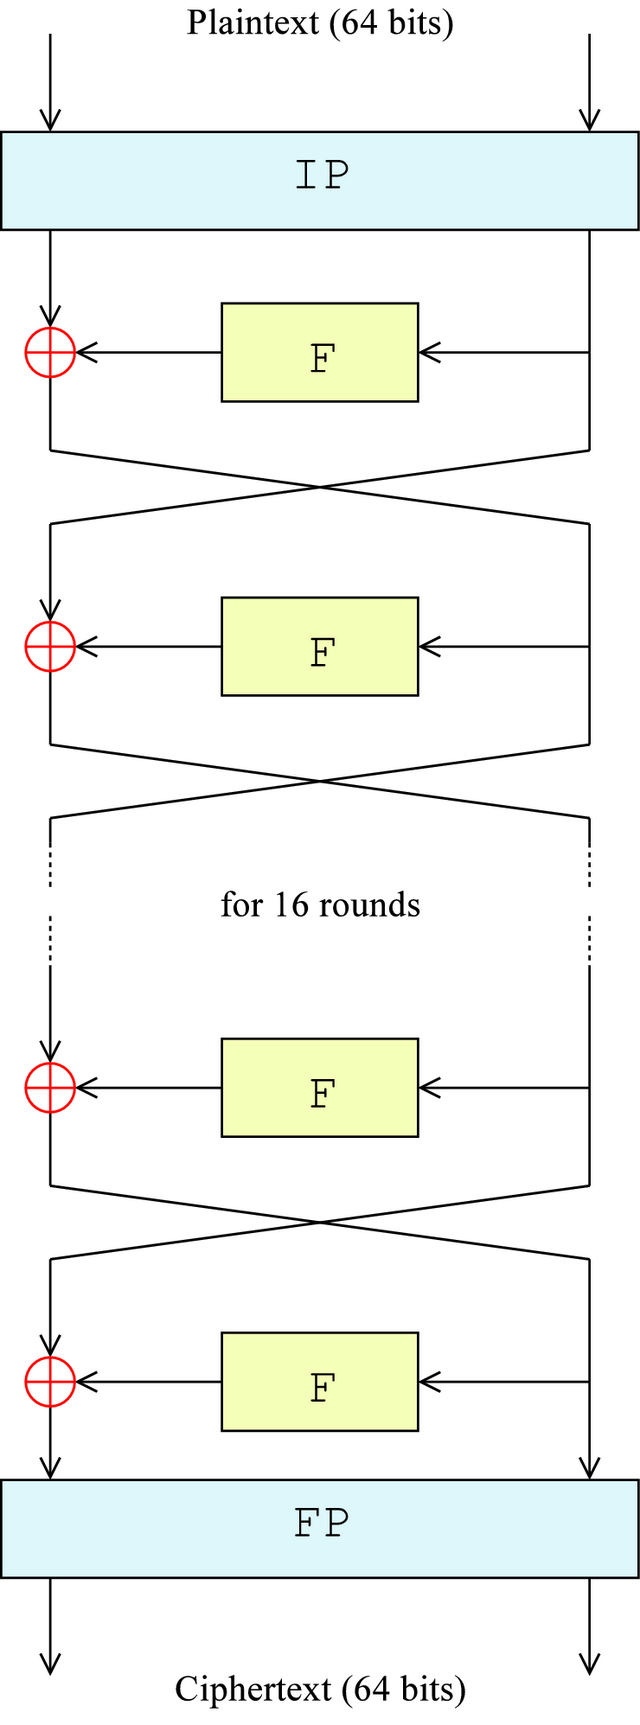
\includegraphics[width=0.33\textwidth]{gfx/feistel_function.png}
    \end{center}
    \caption{Feistel Function}
    \label{fig:feistel}
\end{wrapfigure}

DES defines an encryption method for encrypting 64-bit plain texts using 56-bit keys (the key is 64 bits long, but 8 bits are used for parity). It uses a so-called Feistel function in 16 rounds, where in each round a part of the key is used.

The Feistel function uses another function $F$ to operate on half of the 64-bit block at a time. Its most important characteristic is, that it is reversible, even if the internally used function $F$ is not reversible (e.g. a one-way hash function, which also has collisions).\\
In each iteration of the Feistel function, the plain text will be split in half ($L_i||R_i$) and transformed to a new intermediate ciphertext $L_{i+1}||R_{i+1}$ as follows:

\begin{align*}
    L_{i+1} & := R_i                   \\
    R_{i+1} & := F(k_i,R_i) \oplus L_i
\end{align*}

The exception is the last iteration, in which the sides will not be switched, such that $L{i+1} = F(k_i,R_i) + L_i$ and $R_{i+1} = R_i$.

Regardless of the function $F$, the Feistel function can be reversed by applying it again with reversed key order. That is possible because for each iteration we can compute $L_i$ from $R_{i+1} + L_{i+1}$ and can take $R_i$ directly from $L_{i+1}$.

The Feistel function provides the reversibility of the function, however, it does not provide the security itself. The security is provided by the internally utilized function $F$. In DES this function is using so-called S- and P-boxes, whose details go beyond the scope of this course. What is important, however, is that $F$ implements Shannon's Concept of \textit{confusion and diffusion} and that it takes a part of the key $k_i$ and a bitstring as an input. The function $F$ is, in fact, a non-reversible function.

56 bits ($2^{56}$ possibilities) were soon not sufficient for security against brute-force attackers on modern hardware. What could have been done to increase its security would be creating a new encryption algorithm, which works like DES but uses a longer key. But to reduce the effort required to increase DES's security, another approach was used \textendash{} applying DES multiple times with different keys.

The first approach would be to compute DES two times with two different keys to achieve the security of $2^{112}$, because brute force a ciphertext, the attacker would have to compute all possible combinations of keys of the first DES and keys of the second DES $2^{56} \cdot 2^{56}$. But if an attacker would know the plain text $m$ and the ciphertext $c$ of a message, he could use a \textit{meet-in-the-middle} attack to drastically reduce the computational effort for brute forcing. In the following, the computation of double DES is shown:

$$
    m \rightarrow DES_{1}(key_1, m) \rightarrow c' \rightarrow DES_{2}(key_2, c') \rightarrow c
$$

An attacker could then first compute all possible intermediate ciphertexts $c'$ for all possible values of $k_1$ from $m$ and save the results in a hashmap. Then he could compute all possible intermediate ciphertexts $c'$ with all possible values of $k_2$ from $c$ using $DES_2^{-1}$. The computation required is equal to $2^{56} + 2^{56} = 2 \cdot 2^{56} = 2^{57}$ instead of $2^{112}$. To obtain the correct combination of $k_1$ and $k_2$, the attacker would then search for collisions i.e. for pairs $(k_1, k_2)$ that produced the same intermediate ciphertext $c'$.

For this reason, double DES is not useful. Instead, Triple DES is used, which has the security of $2^{112}$, because the attacker can use a meet-in-the-middle attack but has to calculate two DES on one of the sides. Triple DES uses the inverse operation (reverse order key parts of $k_2$) of $DES_2$ for the second DES. The reason is that there was uncertainty about whether DES could be a \textit{group}, such that there might be one $DES_{x}$ operation, which would be equal to the combination of $DES$ one to three. Later, however, it was discovered, that DES is not a group and inverting the middle DES was, therefore, not required:

$$
    m \rightarrow DES_{1}(key_1, m) \rightarrow c' \rightarrow DES^{-1}_{2}(key_2, c') \rightarrow c'' \rightarrow DES_{3}(key_3, c'') \rightarrow c
$$

%%%%%%%%%%%%%%%%%%%%%%%%%%%%%%%%%%%%%%%%%%%
\section{Advanced Encryption Standard (AES) (Exercise 6)}
%%%%%%%%%%%%%%%%%%%%%%%%%%%%%%%%%%%%%%%%%%%

The security of DES (56-bit keys) and DES3 (112-bit security) is not sufficient. For this reason, the NIST started a public challenge for creating a cryptographic process replacing DES in 1979. The winner of this contest was decided to be Rijndael in 2000, which is the basis for the nowadays used advanced encryption standard (AES). AES is Rijndael, which can generally work with different input and output sizes (block sizes), with a block size of 128-bit. The key length for AES can be chosen to be 128, 192 or 256-bit.

AES is a substitution permutation network. This means it tries to replace bits with other bits (substitution) and change the order of bits (permutation)\footnote{Note that here permutation is a permutation on the set of bits, whereas the \textit{permutation} in PRP refers to a permutation on the set of the different bit strings.}.

AES takes a 128-bit string as input and stores it as a $4 \times 4$ two-dimensional matrix, where each element is an 8-bit substring. Then it executes the following operations on the matrix for a minimum of 10 rounds\footnote{The number of rounds can be greater if longer keys are used.}:

\begin{itemize}
    \item \textit{AddRoundKey:} The round key, which is a substring of the expanded input key, is added ($\oplus$) to the message.
    \item \textit{SubBytes:} Every byte is replaced by another byte according to a fixed replacement scheme (S-box).
    \item \textit{ShiftRows:} The bytes of each row are shifted depending on the row number (row 0 is not shifted, row 1 is shifted 1 element, ...).
    \item \textit{MixColumns:} Same as ShiftRows but for columns.
\end{itemize}

In the last round, AddRoundKey is executed instead of MixColumns. SubBytes is the substitution and ShiftRows and MixColumns are the permutation of the substitution permutation network.

AES is an IND-CPA secure PRP (and therefore also an IND-CPA secure PRF).

%%%%%%%%%%%%%%%%%%%%%%%%%%%%%%%%%%%%%%%%%%%
\section{Block Cipher Modes of Operation (Exercise 6)}
%%%%%%%%%%%%%%%%%%%%%%%%%%%%%%%%%%%%%%%%%%%

The main characteristic of block ciphers is that they can only encrypt bit strings of fixed size.
However, the message size is usually variable and greater than the input size of the block cipher.
Therefore, a method is needed to use block ciphers for messages with arbitrary lengths.
Generally speaking, messages are divided into chunks that match the input length of the block cipher used.
Then the mode of operation provides a schema for the encryption of the individual blocks utilizing a block cipher.
If the message length is not a multiple of the block cipher's input length, padding must be added to the last block of the plain text message before encrypting. Usually, this will be a $1$ followed by the required number of zeroes. This way, the padding can be identified after decrypting by removing all zeroes from the right side until a $1$ appears.

% TODO: add pictures here 

%%%%%%%%%%%%%%%%%%%%%%%%%%%%%%%%%%%%%%%%
\subsection{Electronic Code Book (ECB)}
%%%%%%%%%%%%%%%%%%%%%%%%%%%%%%%%%%%%%%%%

This is the simplest mode of operation. It encrypts every part of the message independently with the same unmodified key. This is not IND-CPA secure, because equal plain text blocks are encrypted to equal ciphertext blocks.\footnote{For formal proof of insecurity, see the solution of exercise sheet 6.}

\begin{figure}
    \center
    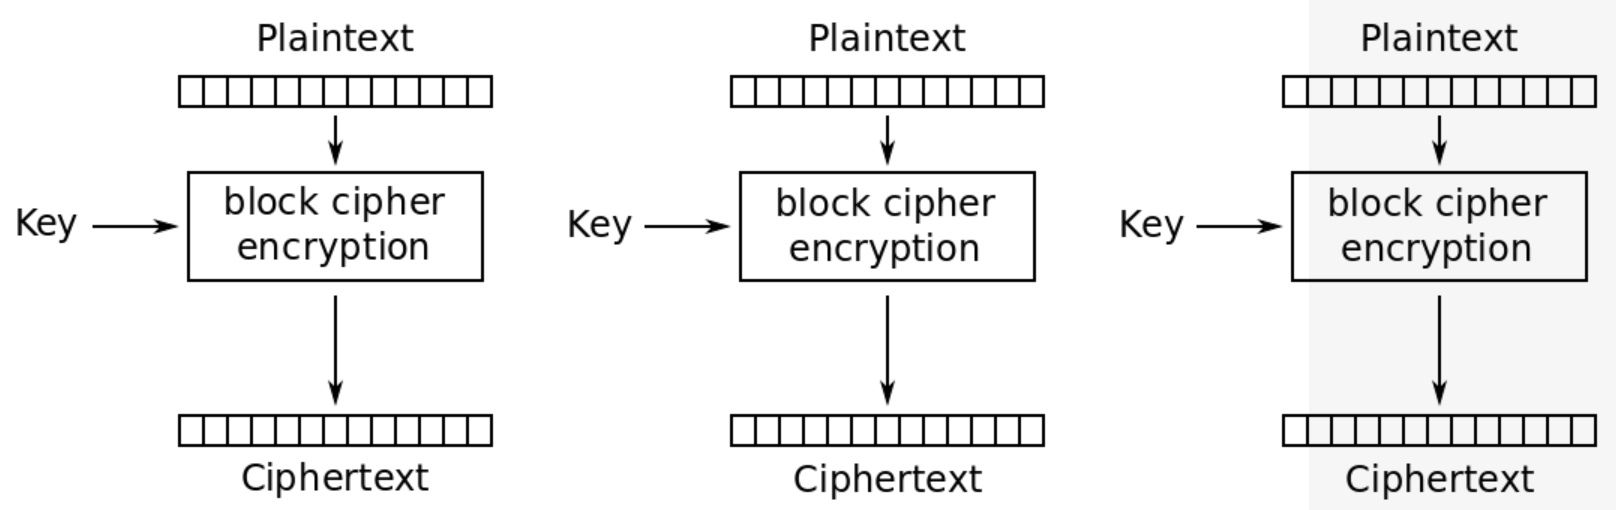
\includegraphics[width=\linewidth]{gfx/ecb_enc_scheme.png}
    \caption{ECB Encryption}
    \label{fig:ecb_enc}
\end{figure}

\begin{figure}
    \center
    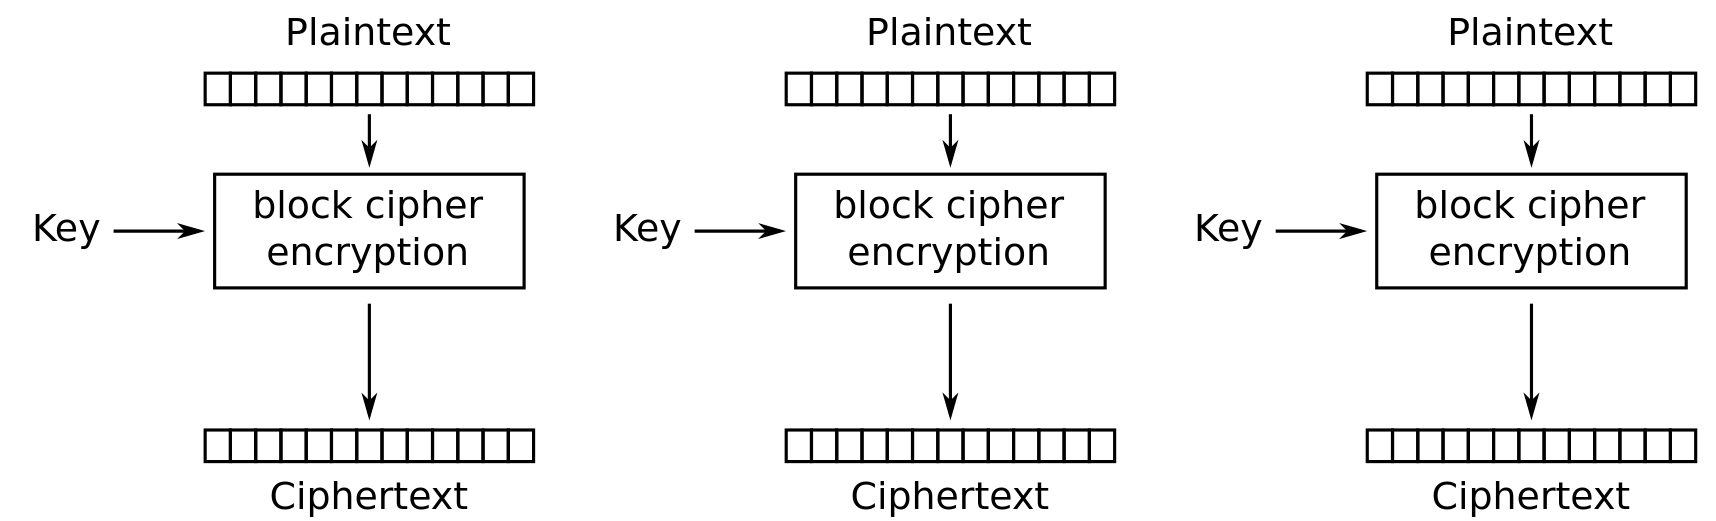
\includegraphics[width=\linewidth]{gfx/ECB_dec_scheme.png}
    \caption{ECB Decryption}
    \label{fig:ecb_dec}
\end{figure}

%%%%%%%%%%%%%%%%%%%%%%%%%%%%%%%%%%%%%%%%
\subsection{Cipher Block Chaining (CBC)}\label{sec:CBC}
%%%%%%%%%%%%%%%%%%%%%%%%%%%%%%%%%%%%%%%%

Cipher block chaining adds ($\oplus$) the previous cipher block to the message before applying the block cipher in each step. Because the cipher blocks are pseudo-random, the input to the block cipher is also pseudo-random, which makes it output pseudo-random. Because for the first block, there is no previous cipher text block, a random initialization vector $IV$ is used. CBC is IND-CPA secure.

\begin{figure}[H]
    \center
    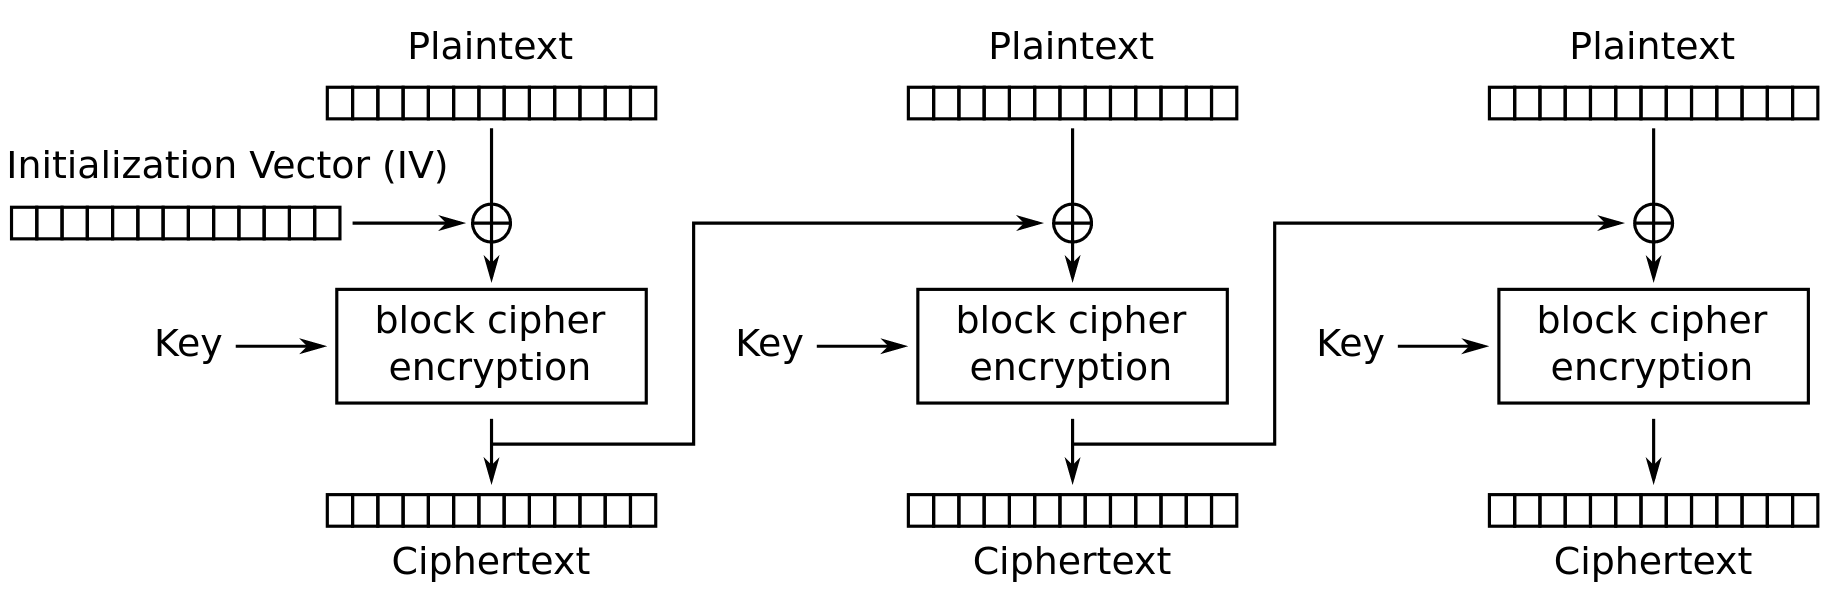
\includegraphics[width=\linewidth]{gfx/CBC_enc_scheme.png}
    \caption{CBC Encryption}
    \label{fig:cbc_enc}
\end{figure}

\begin{figure}[H]
    \center
    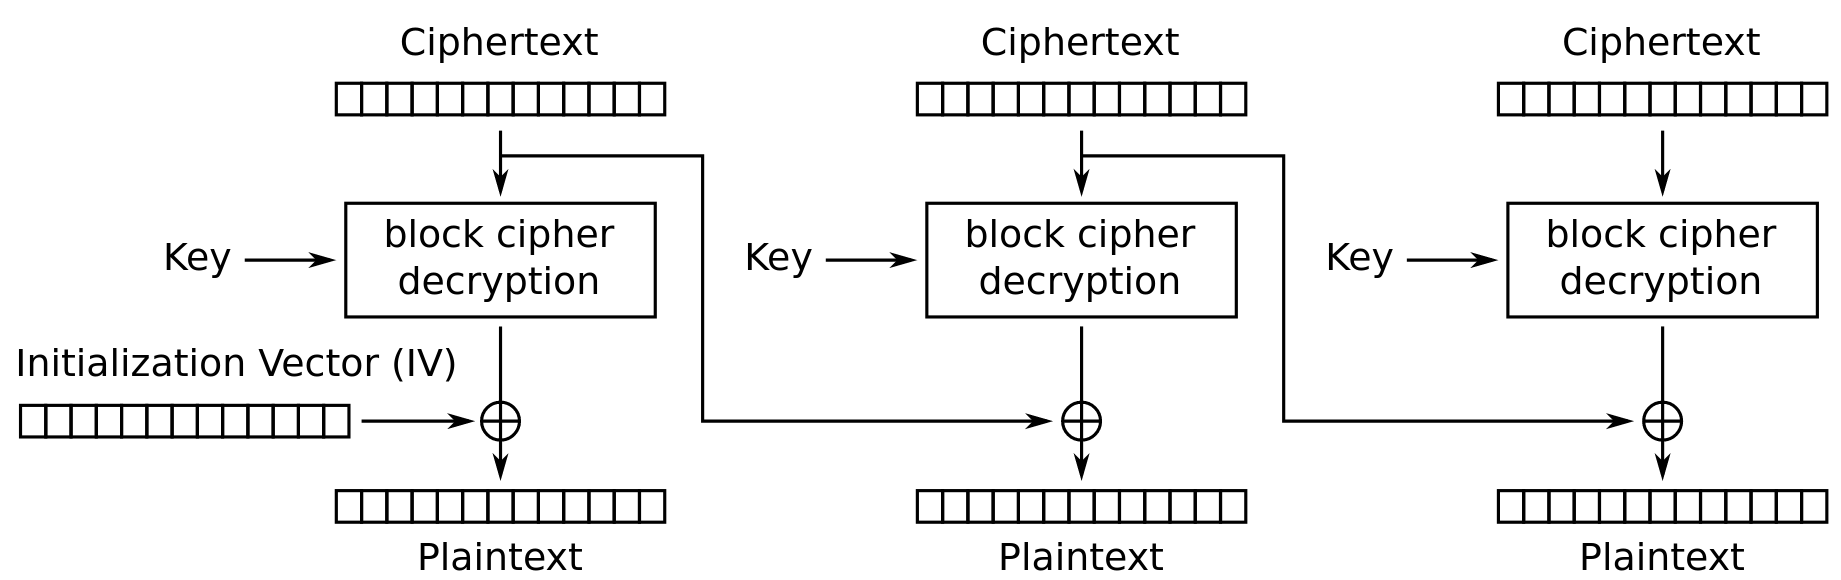
\includegraphics[width=\linewidth]{gfx/CBC_dec_scheme.png}
    \caption{CBC Decryption}
    \label{fig:cbc_dec}
\end{figure}

\textbf{Advantages:}

\begin{itemize}
    \item Parallel Decryption is possible
    \item Loss of a cipher block $c_i$ during transmission only affects plain text blocks $m$ and $m+1$ after decryption (minor advantage)
\end{itemize}

\textbf{Disadvantages:}

\begin{itemize}
    \item Encryption can only happen sequentially
    \item Decryption requires inverse block cipher
\end{itemize}

%%%%%%%%%%%%%%%%%%%%%%%%%%%%%%%%%%%%%%%%
\subsection{Output Feedback Mode (OFB)}
%%%%%%%%%%%%%%%%%%%%%%%%%%%%%%%%%%%%%%%%

The OFB uses the output of the block cipher of the previous iteration as input to the block cipher of each iteration. Because the previous output of the block cipher is pseudo-random, the output of each block cipher is pseudo-random. OFB is IND-CPA secure.

\begin{figure}[H]
    \center
    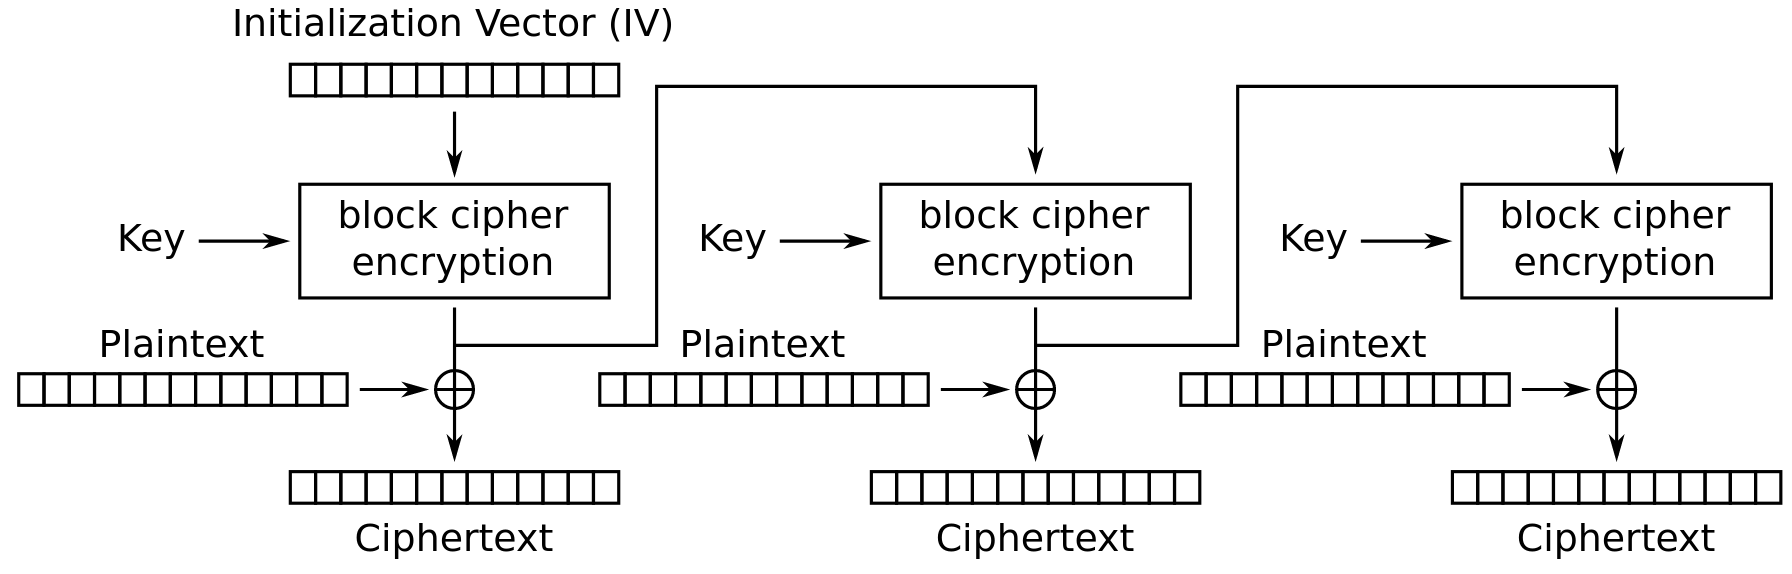
\includegraphics[width=\linewidth]{gfx/OFB_enc_scheme.png}
    \caption{OFB Encryption}
    \label{fig:ofb_enc}
\end{figure}

\begin{figure}[H]
    \center
    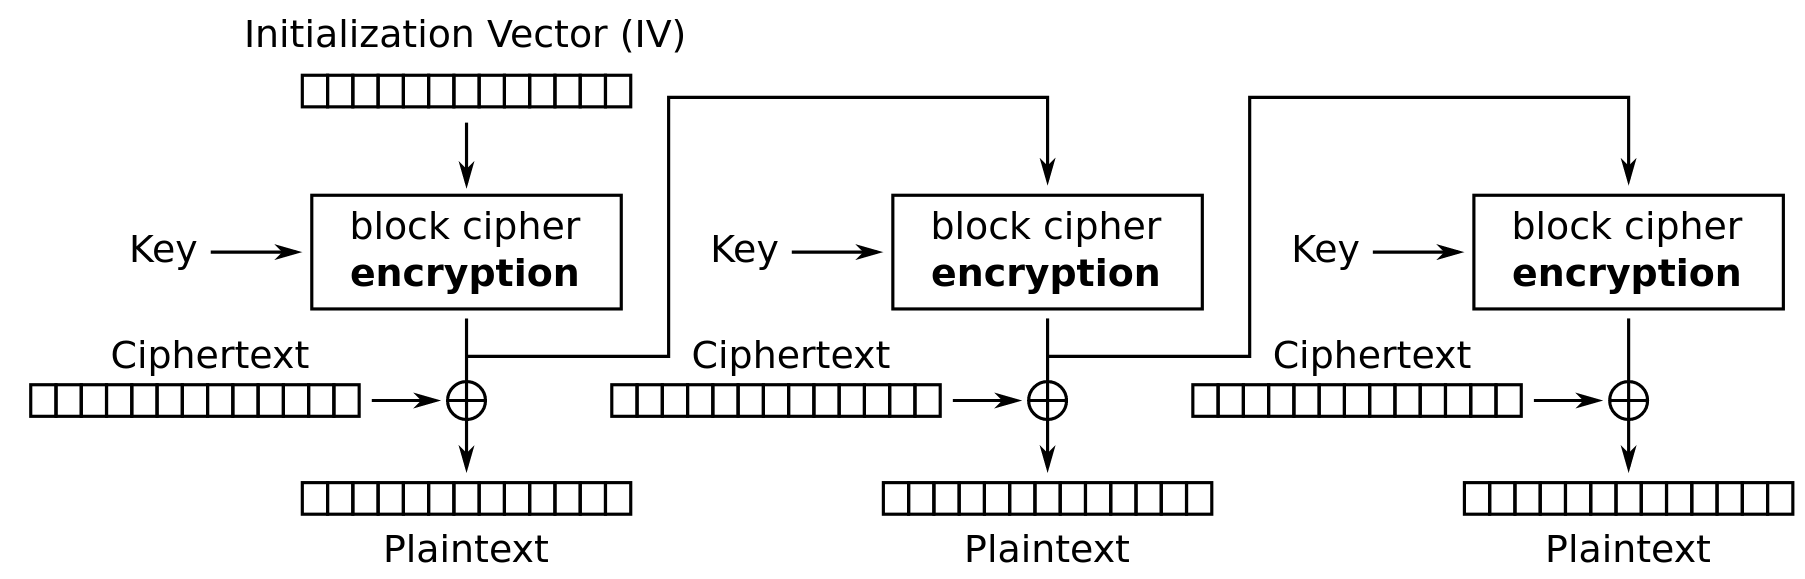
\includegraphics[width=\linewidth]{gfx/OFB_dec_scheme.png}
    \caption{OFB Decryption}
    \label{fig:ofb_dec}
\end{figure}

\textbf{Advantages:}

\begin{itemize}
    \item No inverse operation of the block cipher is required
    \item No padding is required
    \item The block cipher output can be precalculated because it does not depend on the message. As soon as a message arrives, the block-cipher output can be added ($\oplus$) to the message (in parallel possible).
\end{itemize}

\textbf{Disadvantages:}

\begin{itemize}
    \item Encryption and Decryption can only happen sequentially
\end{itemize}

%%%%%%%%%%%%%%%%%%%%%%%%%%%%%%%%%%%%%%%%
\subsection{Cipher Feedback (CFB)}\label{sec:CBF}
%%%%%%%%%%%%%%%%%%%%%%%%%%%%%%%%%%%%%%%%

CFB is a variant of OFB.
Instead of using the output of the block cipher as the input of the next block cipher, the ciphertext block is taken as the next input to the block cipher.
The advantages and disadvantages are the same as those of OFB.

\begin{figure}[H]
    \center
    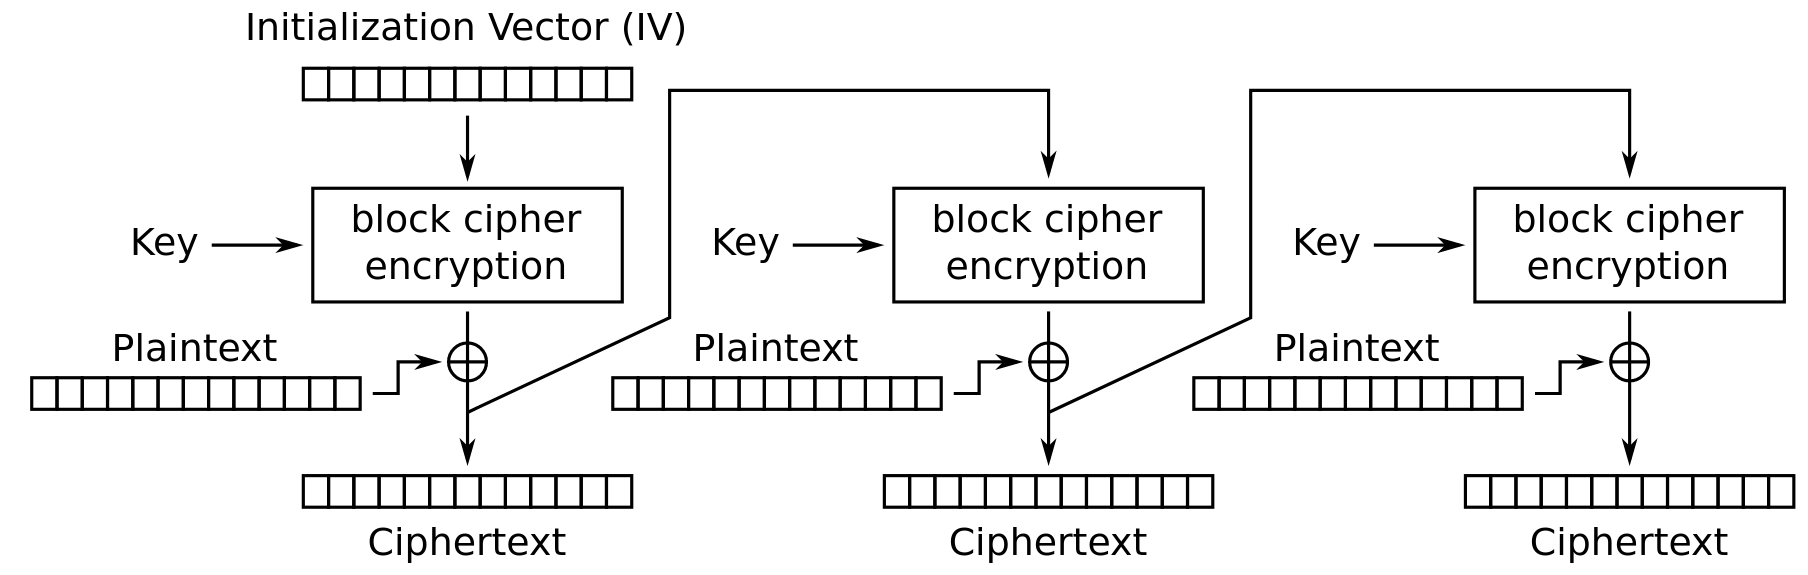
\includegraphics[width=\linewidth]{gfx/cfb_enc.png}
    \caption{CFB Encryption}
    \label{fig:cfb_enc}
\end{figure}

\begin{figure}[H]
    \center
    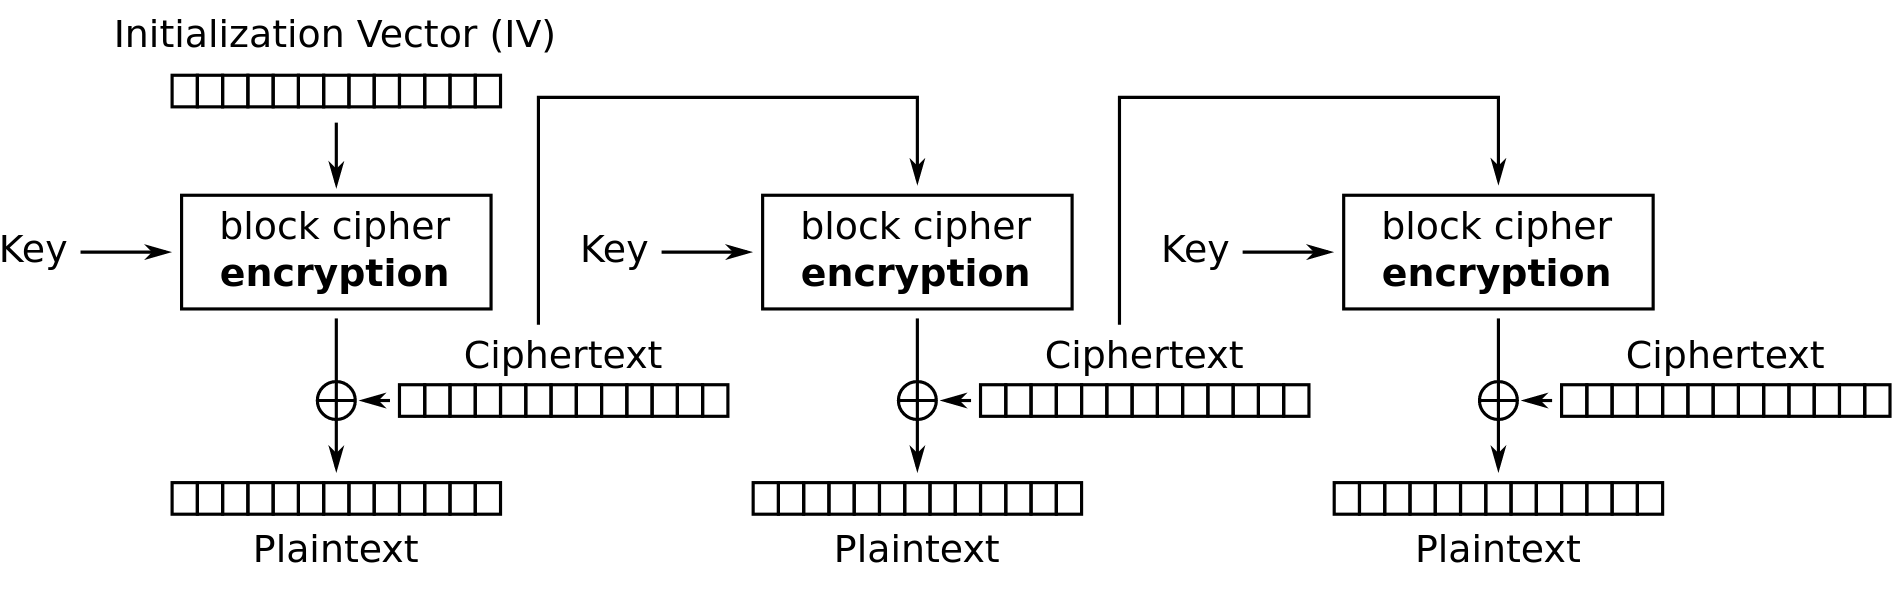
\includegraphics[width=\linewidth]{gfx/cfb_dec.png}
    \caption{CFB Decryption}
    \label{fig:cfb_dec}
\end{figure}

%%%%%%%%%%%%%%%%%%%%%%%%%%%%%%%%%%%%%%%%
\subsection{Counter Mode (CTR)}
%%%%%%%%%%%%%%%%%%%%%%%%%%%%%%%%%%%%%%%%

The counter mode uses a combination of a key (here called initialization vector or Nonce) and a counter.

\begin{figure}[H]
    \center
    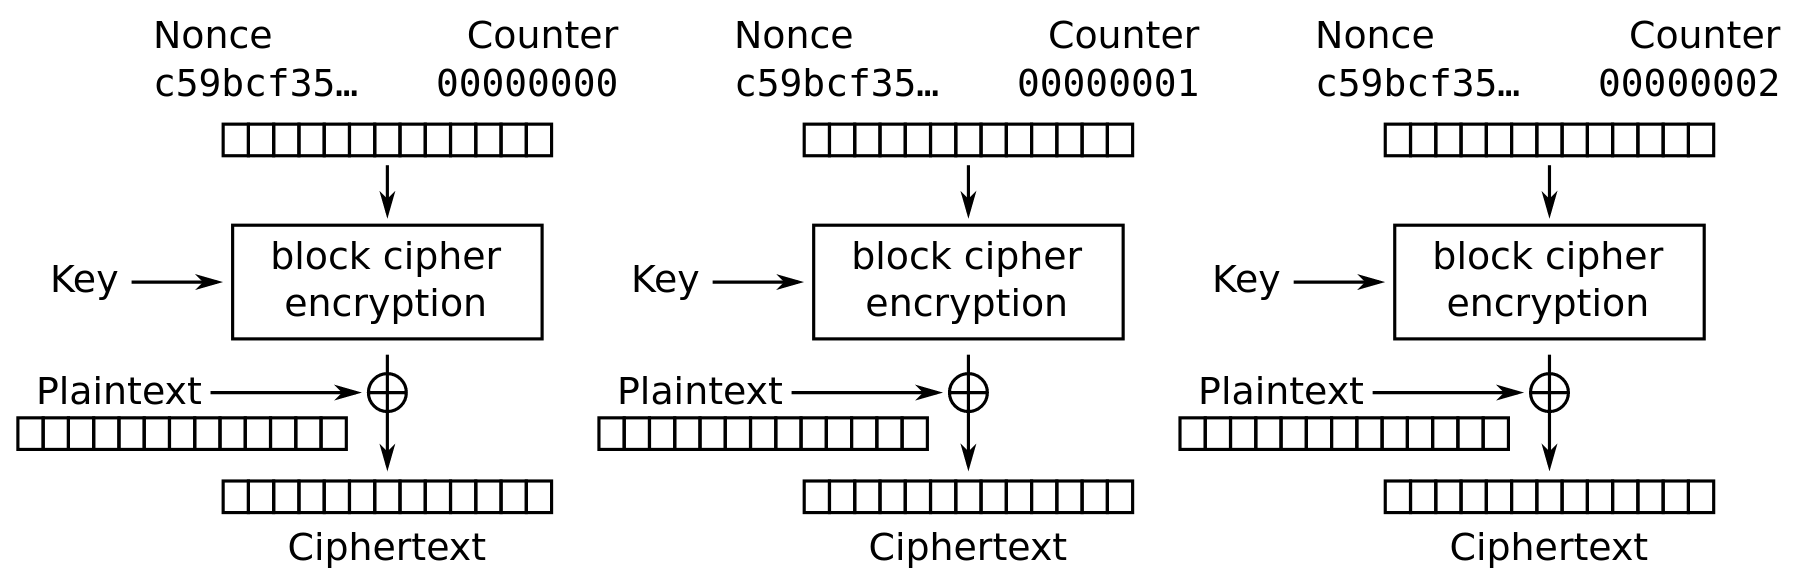
\includegraphics[width=\linewidth]{gfx/enc_ctr.png}
    \caption{CTR Encryption (Decryption analogous, switch plain text and cipher text)}
    \label{fig:ctr_enc}
\end{figure}

\textbf{Advantages:}

\begin{itemize}
    \item Fully parallelizable encryption and decryption
    \item Transmission error in cipher text block $c_i$ only affects plain text block $m_i$
    \item No padding for last plain text block necessary
    \item No inverse operation of the block cipher is required
\end{itemize}

\textbf{Disadvantages:}

\begin{itemize}
    \item Security is reduced by the number of bits that are used as counter bits.
\end{itemize}

%%%%%%%%%%%%%%%%%%%%%%%%%%%%%%%%%%%%%%%%%%%%%%%%
\section{Message Authentication Codes and EUF-CMA}
%%%%%%%%%%%%%%%%%%%%%%%%%%%%%%%%%%%%%%%%%%%%%%%%

Encryption methods only ensure \emph{confidentiality} and are not enough to ensure secure communication. What we want to do is to complement confidentiality with \emph{integrity} and \emph{authenticity}. These properties can be achieved by using \acp{MAC}. \acp{MAC} are checksums that include a secret key in their calculation. That way, if the \ac{MAC} is secure, the receiver of a message can be sure that the message has not been modified if the provided checksum is valid since no attacker can create a matching checksum for a modified message without knowing the secret key.

The security of a \ac{MAC} is defined through the game-based definition of EUF-CMA, which stands for existential unforgeability under chosen message attacks. The attacker $A$ can query as many \acp{MAC} from the \ac{MAC} oracle as it wants. Eventually, $A$ must emit a pair $(m,\tau)$ of a message and a corresponding \ac{MAC}. The attacker $A$ is successful if $\tau$ matches the message $m$ and if the message $m$ has not been queried before.

A slightly stronger variant of EUF-CMA is sEUF-CMA (\emph{strong} EUF-CMA). A \ac{MAC} is sEUF-CMA if the attacker $A$ also wins the game if it finds another \ac{MAC} that is valid for a queried message $m$. That means that the requirements for the attacker's output are less strict. It is not required that the message $m$ has not been queried before, but only that the pair $(m,\tau)$ has not been queried before. Since this gives the attacker additional opportunities to break the \ac{MAC}, the \ac{MAC} must be more secure.

%-------------------------------------------------
\section{PRF-MAC}
%-------------------------------------------------

Every pseudo-random function is also a MAC for messages \emph{with the size of its input length}.
To realize that, the MAC for a message $m$ is calculated by using the PRFs function value at position $m$ using the key $k$ as $MAC := PRF(k,m)$.
To break this MAC an attacker would have to guess the value of a strong PRF without knowing the key, which is not possible.
Hence, the security of PRF-MACs can be proved using a reduction to the IND-CPA security of the used PRF.

%-------------------------------------------------
\section{CBC-MAC}
%-------------------------------------------------

To overcome the limitations that PRF-MAC has for the input message's length, MACs built based on block ciphers can be used.
The block cipher is calculated for the entire message.
Then the last ciphertext block is emitted.
We had seen earlier that the security of block ciphers requires a \emph{random} initialization vector $IV$.
This is different when building MACs based on block ciphers.
Since the first ciphertext block is not transmitted, the receiver would not have a chance to recalculate the MAC as the information about the $IV$ is not transmitted.
One could decide to transmit the $IV$ as well. This, however, would allow the attacker to modify the message and the $IV$, which may allow him to find a matching MAC for the modified message when using the modified $IV$.
Hence, CBC-MACs using random $IV$s and transmitting them are not secure.
Instead, CBC-MACs should use a \emph{constant} $IV$ (usually just $0^\lambda$, which is equivalent to no $IV$).

CBC-MAC (see section \ref{sec:CBC} for details on CBC) is not EUF-CMA if messages with different lengths are allowed because it is vulnerable to length-extension attacks.
In this kind of attack, the attacker chooses a message $m_1$ with the same length as the output of the MAC.
Then the attacker receives $\tau_1$ from the $MAC$ oracle.
Then the attacker sends a second request with $m_2 = \tau_1 \oplus m_1$ to the oracle and receives $\tau_2$.
Now the attacker emits the pair $(m_3 = m_1||m_1,\; \tau_2)$.
$\tau_2$ is a valid MAC for $m_3$, because the CBC-MAC computes
$$\tau_3 = PRF(PRF(m_1) \oplus m_1) = PRF(\tau_1 \oplus m_1) = \tau_2$$
Also, the pair $(m_3,\tau_2)$ is new, because $m_3$ has never been queried before.
Only parts of $m_3$ have been queried.

CMAC is an adapted implementation of CBC-MAC developed by the US government that \emph{is secure} with different message sizes.
To achieve that, CMAC XORs another key to the last plain text block.
This way, the MAC of one message is \emph{not} equal to what the PRF would expect as input for an extended version of the message.

%-------------------------------------------------
\section{HMAC}
%-------------------------------------------------

Another way to construct a MAC is by using hash functions (which will be covered in more detail in a later chapter). The kind of hash function that we want to use is a pseudo-random function (PRF) with much greater output than input length (to compress effectively) and a key length equal to the output length (to chain hash calls by using the output of one iteration as the key for next iteration). This construction is illustrated in Figure \ref{fig:HMAC}. In order to not be vulnerable to length extension attacks it is important to add a \emph{final} step that involves using a different key than the previous steps.

If $f$ is a good PRF, the construction is also a good PRF. Since every good PRF is also a good MAC for a fixed input length, the construction is secure for input messages of the same length.

\begin{figure}[H]
    \center
    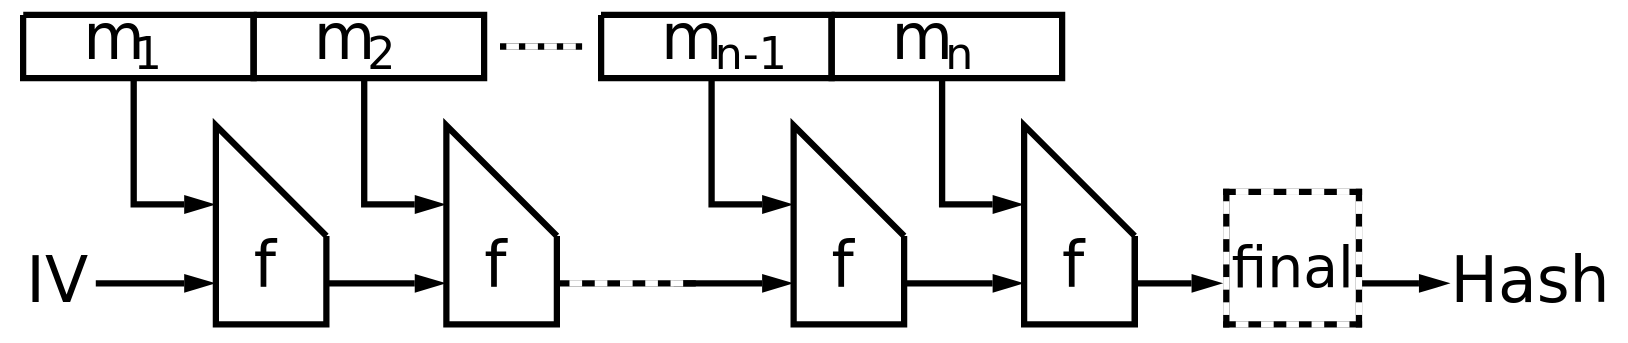
\includegraphics[width=\linewidth]{gfx/HMAC.png}
    \caption{Construction of HMAC using Merkle-Damgard construction.}
    \label{fig:HMAC}
\end{figure}

%++++++++++++++++++++++++++++++++++++++++++++++++++
\section{IND-CCA Security}\label{sec:IND_CCA}
%++++++++++++++++++++++++++++++++++++++++++++++++++

IND-CCA security is a stronger security definition compared to IND-CPA security.
Its security is defined through a game shown in Figure \ref{fig:IND_CCA}.

\begin{figure}[H]
    \center
    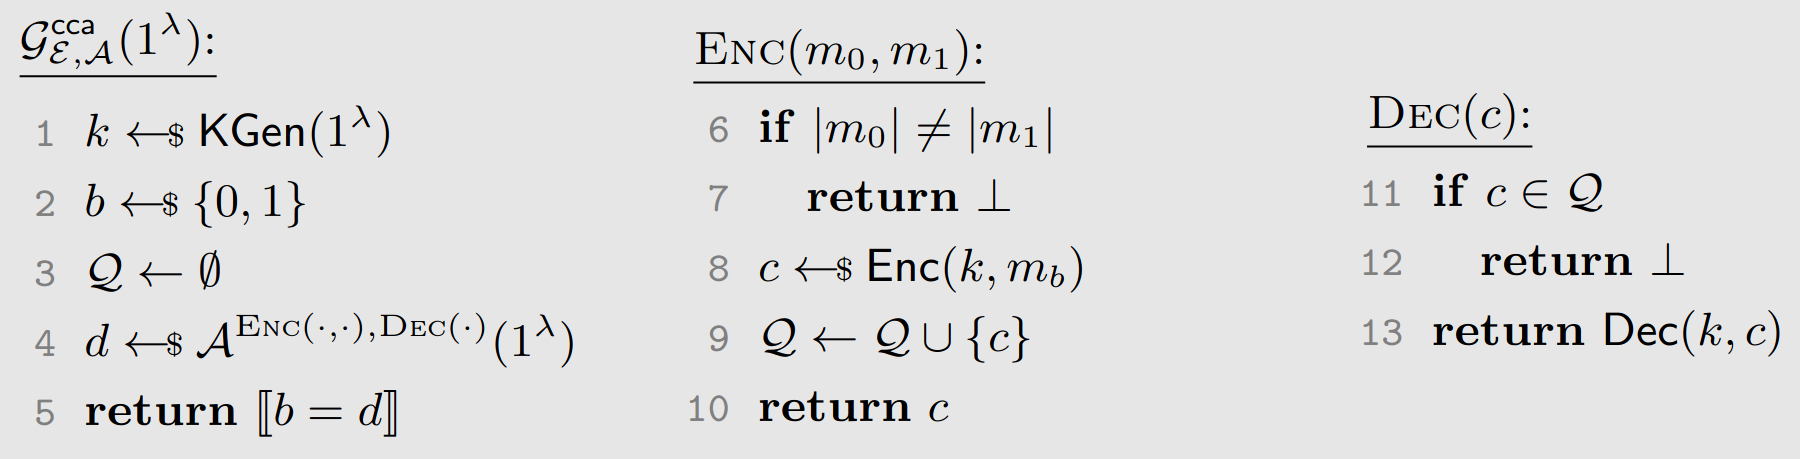
\includegraphics[width=\linewidth]{gfx/IND_CCA.png}
    \caption{Game-based definition of IND-CCA security}
    \label{fig:IND_CCA}
\end{figure}

The attacker has access to two oracles.
The $ENC$ oracle can be queried with two messages $m_0$ and $m_1$ and returns the ciphertext $c_b$ of one of those messages.
Which of the messages is encrypted by a secretly chosen bit $b$ that the attacker $A$ has to be found out by the attacker to be successful.
The $DEC$ oracle can be queried with a ciphertext $c$ and will return the corresponding plain text $m$.
But $DEC$ will only be useful if the same ciphertext $c$ has never been returned by the $ENC$ oracle before.
Because that would make the attack trivial, because the attacker could then obtain a $c_b$ from $ENC$, decrypt it using $DEC$ and obtain $m_b$ and see what message has been encrypted by looking at $m_b$.

Every IND-CCA secure system is also END-CPA secure because not using the $DEC$ oracle is also a valid IND-CCA attack. Using reduction, it can easily be shown that an IND-CPA attacker for $\epsilon$ could be used to break IND-CAA for $\epsilon$, if such an attacker would exist. Therefore, such an attacker cannot exist, which means that $\epsilon$ must be IND-CPA secure if it is IND-CCA secure.

A common way to \emph{construct} an IND-CAA secure system is to use the \emph{Encrypt-then-MAC} scheme.
This scheme first uses an IND-CPA secure encryption mechanism to encrypt a message and then uses an sEUF-CMA secure MAC to tag it.
The encryption output is the combination of the encrypted message and the tag of the ciphertext.
When decrypting, an error is produced if the tag does not match the message's ciphertext.
For this reason, an attacker can not use the $DEC$ oracle in a useful way since he will not obtain an answer unless he forges the tag, which is not possible.
As a result, the attacker effectively only has access to the $ENC$ oracle, which is not sufficient for breaking the system, since the encryption method is IND-CPA secure.
The encrypt-then-MAC construction is shown in its algorithmic representation in Figure \ref{fig:encrypt_then_mac}.

\begin{figure}[H]
    \center
    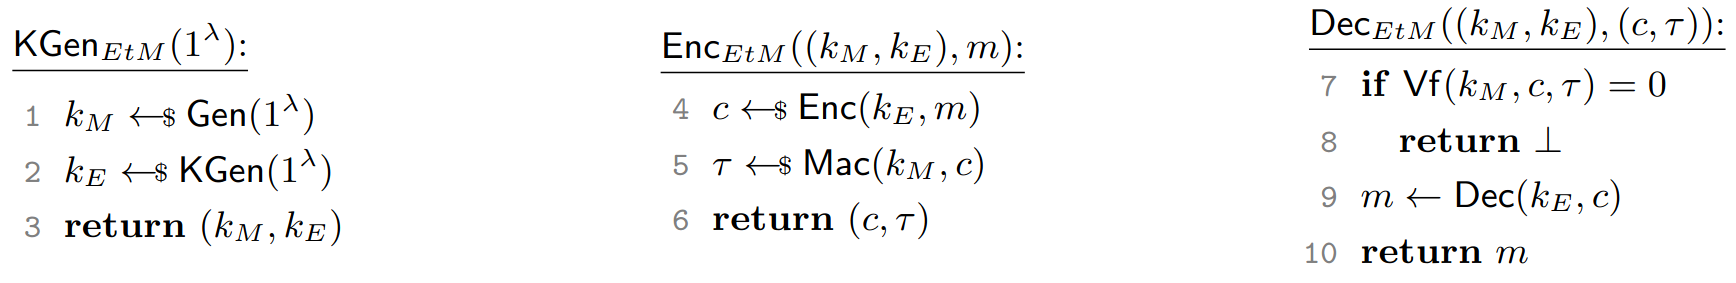
\includegraphics[width=\linewidth]{gfx/EncryptThenMAC.png}
    \caption{Secure encrypt-then-MAC construction based on an IND-CPA secure encryption $Enc$ and decryption $Dec$ and an sEUF-CMA secure MAC ($Mac$ and $Vf$)}
    \label{fig:encrypt_then_mac}
\end{figure}


% TODO: Galois/Counter Mode (if relevant for exam)

